\documentclass{article}
\usepackage[utf8]{inputenc}

\title{Parcial 1}
\author{Nombre: Juan Esteban Cáceres de León}
\date{Carné: 20181049}

\usepackage{natbib}
\usepackage{graphicx}

\begin{document}

\maketitle

\section{Primera serie}

\begin{center}
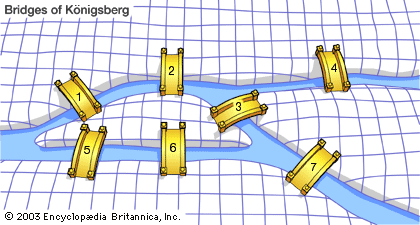
\includegraphics[width=8cm]{bridges.png}
\end{center}
Conjunto de nodos:
\begin{center}
   $Nodos: \{ 1, 2, 3, 4, 5, 6, 7\}$
\end{center}

Conjunto de vértices:

\begin{center}
    $vertices: \{ <1,2> <1,3> <1,4> <1,5> <1,6>
           <2,4> <2,5> <2,6> <2,3> <3,4>
           <3,5> <3,6> <3,7> <4,7> <7,5>
           <7,6> <5,6>$ \}
\end{center}

Grafo representando el conjunto de vértices:

\[
       \left\{
        \begin{array}{l l}
           <1,2> <1,3> <1,4> <1,5> <1,6> \\
           <2,4> <2,5> <2,6> <2,3> <3,4> \\
           <3,5> <3,6> <3,7> <4,7> <7,5> \\
           <7,6> <5,6> \\
        \end{array}
        \right \}
    \]
\section{Segunda serie}
$\frac{n(n+1)}{2}$
\begin{center}
    Caso base: $n = 1$
\end{center}
\begin{center}
    $\frac{1(1 \oplus 1)}{2}$
\end{center}
\begin{center}
    $\frac{2}{2}$
\end{center}
\begin{center}
    $1$
\end{center}
\begin{center}
    Caso inductivo: $n = n \oplus 1$
\end{center}
\begin{center}
    $\frac{(n \oplus 1)((n \oplus 1) \oplus 1)}{2}$
\end{center}
\begin{center}
    $\frac{(n \oplus 1)(n \oplus 2)}{2}$
\end{center}
\begin{center}
    $\frac{(n \oplus 1) }{1}\otimes \frac{(n \oplus 2)}{2}$
\end{center}
\begin{center}
    $\frac{(n \oplus 1) }{1}\otimes (\frac{(n)}{2} \oplus \frac{2}{2})$
\end{center}
\begin{center}
    $\frac{(n \oplus 1) }{1}\otimes (\frac{(n)}{2} \oplus 1)$
\end{center}
\begin{center}
    $\frac{n(n \oplus 1) }{2}\oplus \frac{(n \oplus 1)}{1}$
\end{center}
\begin{center}
    $\frac{n(n \oplus 1) \oplus 2(n \oplus 1)}{2}$
\end{center}
\begin{center}
    $\frac{(n \oplus 1) \otimes (n \oplus 2)}{2}$
\end{center}
\begin{center}
    $\frac{(n \oplus 1)(n \oplus 2)}{2}$
\end{center}
\begin{center}
    $\frac{(n \oplus 1)((n \oplus 1) \oplus 1)}{2}$
\end{center}
\section{Tercera serie}
\[
        \sum(n)=1+2+3+4+\ \ldots\ +n
        \left\{
        \begin{array}{l l}
          \frac{n(n + 1)}{2}
        \end{array}
        \right \}
\]
\begin{center}
   $ \frac{s(0) (s(0) \oplus s(0))}{s(s(0))}$
\end{center}
\begin{center}
    $ \frac{s(0) (s(s(0)))}{s(s(0))}$
\end{center}
\begin{center}
    $ \frac{s(s(0))}{s(s(0))}$
\end{center}
\begin{center}
    $ s(s(0)) \ominus (\frac{s(0)}{s(0)})$
\end{center}
\begin{center}
    $s(s(0)) \ominus s(0)$
\end{center}
\begin{center}
    $s(0)$
\end{center}
\section{Cuarta serie}
$a \oplus b = b \oplus a$
\begin{center}
    caso base: a = 0
\end{center}
\begin{center}
    $0 \oplus b = b \oplus 0$
\end{center}
\begin{center}
   $ b = b$
\end{center}
\begin{center}
    caso inductivo: a = s(i)
\end{center}
\begin{center}
    $s(i) \oplus b = b \oplus s(i)$
\end{center}\begin{center}
    $s(i \oplus b) = s(b \oplus i)$
\end{center}\begin{center}
    $s(i \oplus b) = s(i \oplus b)$
\end{center}
\section{Quinta serie}
$((n \oplus n) \geq n) = s(0)$
\begin{center}
    caso base: n = 0
\end{center}
\begin{center}
    $((0 \oplus 0) \geq 0)$
\end{center}
\begin{center}
    $0 \geq 0$
\end{center}
\begin{center}
    caso inductivo: n = s(0)
\end{center}
\begin{center}
    $((s(0) \oplus s(0)) \geq s(0))$
\end{center}
\begin{center}
    $((s(s(0 \oplus 0))) \geq s(0))$
\end{center}
\begin{center}
    $((s(s(0))) \geq s(0))$
\end{center}
\begin{center}
    $(s(s(0)) \ominus s(0) \geq 0)$
\end{center}
\begin{center}
    $(s(0) \geq 0)$
\end{center}
\begin{center}
    $(((n \oplus n) \geq n) = s(0)) = s(0)$
\end{center}


\end{document}
